\documentclass[12pt]{exam}
\usepackage[utf8]{inputenc}		% Caracteres latinos
\usepackage[spanish]{babel}		% Idioma español
\usepackage{geometry}			% Organizar el documento
\usepackage{graphicx}			% Incluir gráficos
\usepackage{makecell}			% Para personalizar las celdas de una tabla
\usepackage[nohdr]{mathexam}	% Añadimos el paquete mathexam (sin header)
\usepackage{amsmath}
\usepackage{amsfonts}
\usepackage{amssymb}
\usepackage{mathtools}
\usepackage{tikz}
\usepackage{pgfplots}
\pgfplotsset{compat=1.10}
\usepgfplotslibrary{fillbetween}
%\usetikzlibrary{positioning}    % yo
\usepgfplotslibrary{polar}
\usepackage[shortlabels]{enumitem}
\renewcommand{\baselinestretch}{1.5}
\usepackage{mathtools}
\usepackage{bm}
\usepackage{esvect}
\usepackage[fleqn]{mathtools}
\usepackage{relsize}
\usepackage{multirow}
\usepackage{multicol}
\usepackage[document]{ragged2e}
\usepackage{textpos}
\usepackage{tcolorbox}
\usepackage{hyperref}
\usepackage{enumerate}
\usetikzlibrary{3d}
\usepackage{pgfplotstable}
\pgfplotsset{compat=1.18}
%% \usepackage{wrapfig} % wrapfigure
%% \usepackage{float}
%% \usepackage{graphicx}
\usepackage{here} % [H]
\spanishdecimal{.}


\geometry{
  a4paper,                    % Tamaño del documento
  hmargin = {1.7cm, 1.7cm}, 	% Margen horizontal izquierdo, derecho
  vmargin = {1cm, 1cm},	    % Margen vertical superior, inferior
  headsep = 4mm,				% Separación entre el encabezado y el texto
  head = .2cm,				% Tamaño del encabezado
  % marginparsep = 5mm, 		% Seperación entre las notas y el texto
  % marginpar = 1.5cm,		% Tamaño de las notas
  includeall,                 % incluye el encabezado, footer y notas dentro del tamaño del documento
  nomarginpar,	            % Elimina las notas
  foot = 1cm,                 % Tamaño del footer
  twoside,                	% Habilita el modo de impresión a doble cara
}

\selectlanguage{spanish}       
\spanishdecimal{.}

\newcommand{\iuni}{\pmb{\hat{\imath}}}
\newcommand{\juni}{\pmb{\hat{\jmath}}}
\newcommand{\kuni}{\pmb{\hat{k}}}
% DOCUMENTO


\begin{document}

\centering

\Large 
\textbf{Tarea A}\\
\large 
Unidad 2: Integrales triples y aplicaciones \\
Alumno: Zarco Romero José Antonio\\
Valor: 6 puntos\\
\normalsize
Fecha de entrega: 

Miércoles 18/09/2024 durante la clase

\vskip10pt

\normalsize

\pointpoints{punto}{puntos}
\pointformat{\bfseries\boldmath(\thepoints)}
\vskip10pt

\begin{questions}

  \question{Evalúa las integrales iteradas.}

  \begin{enumerate}[(a)]
  \item $\int_0^1 \int_0^z \int_0^{x+z} 6xz ~ dy ~ dx ~ dz$

    \begin{align*}
      \int_0^1 \int_0^z \int_0^{x+z} 6xz ~ dy ~ dx ~ dz
      &= \int_0^1 \int_0^z 6xz \left[\int_0^{x+z} ~ dy\right] ~ dx ~ dz \\
      &= \int_0^1 \int_0^z 6xz \left[y\right]_0^{x+z} ~ dx ~ dz \\
      &= \int_0^1 \int_0^z 6xz(x+z) ~ dx ~ dz \\
      &= \int_0^1 \left[ \int_0^z 6x^2z + 6xz^2 ~ dx \right] ~ dz \\
      &= \int_0^1 6z \left[ \int_0^z x^2 + xz ~ dx \right] ~ dz \\
      &= \int_0^1 6z \left[ \frac{x^3}{3} + \frac{x^2z}{2} \right]_0^z ~ dz \\
      &= \int_0^1 6z \left[ \frac{z^3}{3} + \frac{z^3}{2} \right] ~ dz \\
      &= \int_0^1 6z \left[ \frac{5z^3}{6} \right] ~ dz \\
      &= \int_0^1 5z^4 ~ dz \\
      &= \left[ \frac{5z^5}{5} \right]_0^1 \\
      &= 1^5 - 0^5 \\
      &= 1
    \end{align*}

    $\therefore \quad \int_0^1 \int_0^z \int_0^{x+z} 6xz ~ dy ~ dx ~ dz = 1$

  \item $\int_0^3 \int_0^1 \int_0^{sqrt{1-z^2}} ze^y ~ dx ~ dz ~ dy$

    \begin{align*}
      \int_0^3 \int_0^1 \int_0^{sqrt{1-z^2}} ze^y ~ dx ~ dz ~ dy
      &= \int_0^3 \int_0^1 ze^y \left[ \int_0^{\sqrt{1-z^2}} ~ dx \right] ~ dz ~ dy \\
      &= \int_0^3 \int_0^1 ze^y \left[ x \right]_0^{\sqrt{1-z^2}} ~ dz ~ dy \\
      &= \int_0^3 \int_0^1 ze^y \sqrt{1-z^2} ~ dz ~ dy \\
      &= \int_0^3 e^y \left[ \int_0^1 z \sqrt{1-z^2} ~ dz \right] ~ dy
    \end{align*}

    Sea $u=1-z^2$, entonces $\frac{du}{dz} = -2z \Rightarrow -\frac{du}{2} = z ~ dz$. Además,
    $u(0) = 1$ y $u(1) = 0$. Por lo tanto,

    \begin{align*}
      \int_0^3 \int_0^1 \int_0^{\sqrt{1-z^2}} ze^y ~ dx ~ dz ~ dy
      &= \int_0^3 e^y \left[ -\frac{1}{2} \int_1^0 \sqrt{u} ~ du \right] ~ dy \\
      &= \int_0^3 e^y \left[ \frac{1}{2} \int_0^1 u^{1/2} ~ du \right] ~ dy \\
      &= \int_0^3 e^y \left[ \frac{1}{2} \left( \frac{2}{3} u^{3/2} \right)_0^1 \right] ~ dy \\
      &= \int_0^3 e^y \left[ \frac{1}{3} \right] ~ dy \\
      &= \frac{1}{3} \int_0^3 e^y ~ dy \\
      &= \frac{1}{3} \left[ e^y \right]_0^3 \\
      &= \frac{1}{3} \left( e^3 - e^0 \right) \\
      &= \frac{1}{3} \left( e^3 - 1 \right)
    \end{align*}

    $\therefore \quad \int_0^3 \int_0^1 \int_0^{\sqrt{1-z^2}} ze^y ~ dx ~ dz ~ dy = \frac{1}{3} \left( e^3 - 1 \right)$
  \end{enumerate}

  \question{Usa una triple integral para encontrar el volumen del tetraedro encerrado por los planos coordenados y el plano $2x+y+z=4$.}

  El tetraedro está encerrado por los planos $x=0$, $y=0$, $z=0$ y $2x+y+z=4$. Por lo que, intersecta a los planos coordenados

  \begin{enumerate}
  \item $xy ~(z=0)$ en 
    \begin{align*}
      2x+y &= 4 \\
      y &= 4-2x
    \end{align*}
    Intersecta a $x=0$ en $y=4$ y a $y=0$ en $x=2$, es decir, $(0,4,0)$ y $(2,0,0)$.
    
  \item $xz ~(y=0)$ en 
    \begin{align*}
      2x+z &= 4 \\
      z &= 4-2x
    \end{align*}
    Intersecta a $x=0$ en $z=4$ y a $z=0$ en $x=2$, es decir, $(0,0,4)$ y $(2,0,0)$.

  \item $yz ~(x=0)$ en
    \begin{align*}
      y+z &= 4 \\
      z &= 4-y
    \end{align*}
    Intersecta a $y=0$ en $z=4$ y a $z=0$ en $y=4$, es decir, $(0,0,4)$ y $(0,4,0)$.

  \end{enumerate}

  De modo que, la región sólida $E$ está dada por

  \begin{figure}[H]
    \centering
    \begin{tikzpicture}
      \begin{axis}[
          view={120}{30},
          axis lines=center,
          axis on top,
          xlabel={$x$},
          ylabel={$y$},
          zlabel={$z$},
          xtick={1},
          ytick={1},
          ztick={1},
          xticklabels={$1$},
          yticklabels={$1$},
          zticklabels={$1$},
          no marks,
        ]
        
        % Dibujar planos
        \addplot3[fill=blue, opacity=0.1] coordinates {(0,0,0) (0,0,4) (0,4,0) (4,0,0) (0,0,0)};
        \addplot3[fill=blue, opacity=0.1] coordinates {(0,0,0) (0,0,4) (4,0,0) (0,0,0)};
        \addplot3[fill=blue, opacity=0.1] coordinates {(0,0,0) (0,4,0) (4,0,0) (0,0,0)};
        \addplot3[fill=blue, opacity=0.1] coordinates {(0,0,4) (0,4,0) (4,0,0) (0,0,4)};
        
        % Dibujar líneas de los ejes
        \draw[thick,->] (axis cs: -4,0,0) -- (axis cs: 8,0,0) node[anchor=north] {};
        \draw[thick,->] (axis cs: 0,-4,0) -- (axis cs: 0,8,0) node[anchor=south] {};
        \draw[thick,->] (axis cs: 0,0,-4) -- (axis cs: 0,0,8) node[anchor=west] {};

        % Coordenadas de intersección
        \node[anchor=south] at (axis cs: 0,3,0) {$(0,4,0)$};
        \node[anchor=south] at (axis cs: 3,0,0) {$(2,0,0)$};
        \node[anchor=south] at (axis cs: 0,0,3) {$(0,0,4)$};
      \end{axis}
    \end{tikzpicture}
    \caption{Región sólida $E$}
  \end{figure}

  Y, la proyección $D$ sobre el plano $xy$ es

  \begin{figure}[H]
    \centering
    \begin{tikzpicture}
      \begin{axis}[
          axis lines = center,
          xlabel = {$x$},
          ylabel = {$y$},
          xtick = {0, 2},
          ytick = {0, 4},
          ymin = 0,
          ymax = 5,
          xmin = 0,
          xmax = 3,
          samples = 100,
          domain = 0:2,
          fill=gray,
          axis on top,
        ]

        % Dibujar la función y = 4 - 2x
        \addplot[thick,blue,domain=0:2] {4 - 2*x};

        % Sombrear la región bajo la curva
        \addplot [domain=0:2,fill=blue,opacity=0.1] {4-2*x} \closedcycle;

        % Etiquetas
        \node at (axis cs: 2, 0) [anchor=north] {$(2, 0)$};
        \node at (axis cs: 0, 4) [anchor=east] {$(0, 4)$};

        %Ecuación
        \node at (axis cs: 2, 2) [anchor=north] {$2x + y = 4$};
      \end{axis}
    \end{tikzpicture}
    \caption{Proyección $D$ sobre el plano $xy$}
  \end{figure}

  La cota inferior del tetaedro es $z=0$ y la cota superior es el plano $2x+y+z=4$ (o $z=4-2x-y$). Observe que los planos $2x+y+z=4$ y $z=0$ se cortan en la recta $2x+y=4$ (o $y=4-2x$) 
  en el plano $xy$. Por consiguiente, la proyección de $E$ es la región triangular $D$, y se tiene

  \[
  E = \{ (x,y,z) \in \mathbb{R}^3 \mid 0 \leq x \leq 2, 0 \leq y \leq 4-2x, 0 \leq z \leq 4-2x-y \}
  \]

  Esta descripción de $E$ como una región de \textbf{tipo I} permite evaluar la integral como sigue:

  Recordemos que

  \begin{tcolorbox}[colback=white, colframe=blue!40!black, title=\textbf{Volumen de un sólido}]
    El volumen de un sólido $E$ en el espacio tridimensional es

    \[
    V(E) = \iiint_E dV
    \]
  \end{tcolorbox}

  \begin{align*}
    \iiint_E dV 
    &= \int_0^2 \int_0^{4-2x} \int_0^{4-2x-y} dz ~ dy ~ dx \\
    &= \int_0^2 \int_0^{4-2x} \left[ \int_0^{4-2x-y} ~ dz \right] ~ dy ~ dx \\
    &= \int_0^2 \int_0^{4-2x} \left[ z \right]_0^{4-2x-y} ~ dy ~ dx \\
    &= \int_0^2 \int_0^{4-2x} (4-2x-y) ~ dy ~ dx \\
    &= \int_0^2 \left[ \int_0^{4-2x} 4-2x-y~ dy \right] ~ dx \\
    &= \int_0^2 \left[ 4y-2xy-\frac{y^2}{2} \right]_0^{4-2x} ~ dx \\ 
    &= \int_0^2 \left[ 4(4-2x)-2x(4-2x)-\frac{(4-2x)^2}{2} \right] ~ dx \\
    &= \int_0^2 \left[ 16-8x -8x+4x^2- \left(\frac{16-16x+4x^2}{2}\right) \right] ~ dx \\
    &= \int_0^2 \left[ 16-16x+4x^2-8+8x-2x^2 \right] ~ dx \\ %bien
    &= \int_0^2 \left[ 8-8x+2x^2 \right] ~ dx \\
    &= \left[ 8x-4x^2+\frac{2x^3}{3} \right]_0^2\\
    &= 8(2)-4(4)+\frac{2(8)}{3}  
  \end{align*}
  \begin{align*}
    \iiint_E dV 
    &= 16-16+\frac{16}{3} \\
    &= \frac{16}{3}
  \end{align*}

  $\therefore$ El volumen del tetraedro encerrado por los planos coordenados y el plano $2x+y+z=4$ es de $\frac{16}{3}$ unidades cúbicas.

  \question{Expresa la integral $\iiint_E f(x,y,z) ~ dV$ como una integral iterada en seis diferentes formas, donde $E$ es el sólido delimitado por las superficies $x^2+z^2=4$, $y=0$ y $y=6$.}

  \begin{figure}[H]
    \centering
    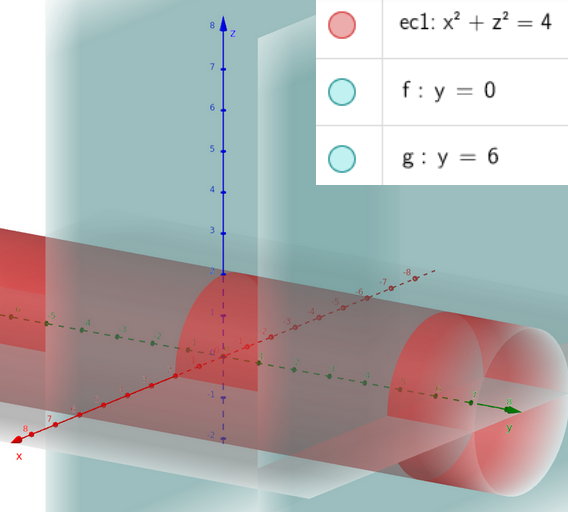
\includegraphics[width=10cm]{../img/t2a/t2a_ej3.png}
    \caption{Región sólida $E$}
  \end{figure}
  
  Veamos como son las proyecciones del sólido $E$ en los planos:

  \begin{enumerate}
  \item $xy ~ (z=0)$.
    \[
    D_1 = \left\{ (x,y)~|~ -2 \leq x \leq 2, 0 \leq y \leq 6 \right\}
    \]

    \begin{figure}[H]
      \centering
      \begin{tikzpicture}
        
        % Rectángulo iluminado
        \filldraw[fill=yellow!30, draw=black] (-2,0) rectangle (2,6);
        
        % Etiquetas de los vértices
        \node at (-2,0.5) {(-2, 0)};
        \node at (2,0.5) {(2, 0)};
        \node at (-2,6.3) {(-2, 6)};
        \node at (2,6.3) {(2, 6)};
        
        % División de los ejes
        \foreach \x in {-2,-1,1,2}
        \draw (\x,0.1) -- (\x,-0.1) node[below] {\x};
        \foreach \y in {0,2,4,6}
        \draw (0.1,\y) -- (-0.1,\y) node[left] {\y};
        
        % Ejes
        \draw[->] (-3,0) -- (3,0) node[right] {$x$};
        \draw[->] (0,-1) -- (0,7) node[above] {$y$};
      \end{tikzpicture}
      \caption{Proyección $D_1$ de $E$ en el plano $xy$}
    \end{figure}

  \item $yz ~ (x=0)$
    \[
    D_2 = \left\{ (y,z) ~|~  -2 \leq z \leq 2, 0 \leq y \leq 6 \right\}
    \]

    \begin{figure}[H]
      \centering
      \begin{tikzpicture}
        
        % Rectángulo iluminado
        \filldraw[fill=yellow!30, draw=black] (0,-2) rectangle (6,2);
        
        % Etiquetas de los vértices
        \node at (0.8,-1.5) {(0, -2)};
        \node at (0.8,1.5) {(0, 2)};
        \node at (5,-1.5) {(6, -2)};
        \node at (5,1.5) {(6, 2)};
        
        %% % División de los ejes
        \foreach \y in {-2,-1,1,2}
        \draw (0.1,\y) -- (-0.1,\y) node[left] {\y};
        \foreach \x in {0,2,4,6}
        \draw (\x,0.1) -- (\x,-0.1) node[below] {\x};
        
        % Ejes
        \draw[->] (-1,0) -- (7,0) node[right] {$y$};
        \draw[->] (0,-3) -- (0,3) node[above] {$z$};
        
      \end{tikzpicture}
      \caption{Proyección $D_2$ de $E$ en el plano $yz$}
    \end{figure}

  \item $xz ~ (y=0)$
    \[
    D_3 = \left\{ (x,z) ~|~ x^2+y^2 \leq 4 \right\}
    \]

    \begin{figure}[H]
      \centering
      \begin{tikzpicture}
        
        % Círculo iluminado
        \filldraw[fill=yellow!30, draw=black] (0,0) circle (2);
        
        % Etiquetas de la circunferencia
        \node at (2.5,0.5) {$(2, 0)$};
        \node at (-2.7,0.5) {$(-2, 0)$};
        \node at (0,2.5) {$(0, 2)$};
        \node at (0,-2.5) {$(0, -2)$};
        
        % División de los ejes
        \foreach \x in {-2,-1,1,2}
        \draw (\x,0.1) -- (\x,-0.1) node[below] {\x};
        \foreach \z in {-2,-1,1,2}
        \draw (0.1,\z) -- (-0.1,\z) node[left] {\z};
        % Ejes
        \draw[->] (-3,0) -- (3,0) node[right] {$x$};
        \draw[->] (0,-3) -- (0,3) node[above] {$z$};
        
      \end{tikzpicture}
      \caption{Proyección $D_3$ de $E$ en el plano $xz$}
    \end{figure}
  \end{enumerate}

  Entonces,
  
  \begin{enumerate}
  \item \textbf{Sólido Tipo 1}
    \begin{align*}
      E &= \left\{ (x,y,z) ~|~ (x,y) \in D_1, u_1(x,y) \leq z \leq u_2(x,y) \right\}
    \end{align*}
    donde $u_1(x,y) = -\sqrt{4-x^2}$ y $u_2(x,y) = \sqrt{4-x^2}$.

    Si $D_1$ es 

    \begin{itemize}
    \item $y-$simple
      \begin{align*}
        E &= \left\{ (x,y,z) ~|~ -2 \leq x \leq 2, 0 \leq y \leq 6, -\sqrt{4-x^2} \leq z \leq \sqrt{4-x^2} \right\}
      \end{align*}

    \item $x-$simple
      \begin{align*}
        E &= \left\{ (x,y,z) ~|~ -2 \leq x \leq 2, 0 \leq y \leq 6, -\sqrt{4-x^2} \leq z \leq \sqrt{4-x^2} \right\}
      \end{align*}
    \end{itemize}

  \item \textbf{Sólido Tipo 2}
    \begin{align*}
      E &= \left\{ (x,y,z) ~|~ (y,z) \in D_2, u_1(y,z) \leq x \leq u_2(y,z) \right\}
    \end{align*}
    donde $u_1(y,z) = -\sqrt{4-z^2}$ y $u_2(y,z) = \sqrt{4-z^2}$.

    Si $D_2$ es 

    \begin{itemize}
    \item $y-$simple
      \begin{align*}
        E &= \left\{ (x,y,z) ~|~ -\sqrt{4-z^2} \leq x \leq \sqrt{4-z^2}, 0 \leq y \leq 6, -2 \leq z \leq 2 \right\}
      \end{align*}

    \item $z-$simple
      \begin{align*}
        E &= \left\{ (x,y,z) ~|~ -\sqrt{4-z^2} \leq x \leq \sqrt{4-z^2}, 0 \leq y \leq 6, -2 \leq z \leq 2 \right\}
      \end{align*}
    \end{itemize}

  \item \textbf{Sólido Tipo 3}
    \begin{align*}
      E &= \left\{ (x,y,z) ~|~ (x,z) \in D_3, u_1(x,z) \leq y \leq u_2(x,z) \right\}
    \end{align*}
    donde $u_1(x,z) = 0$ y $u_2(x,z) = 6$.

    Si $D_3$ es 
    
    \begin{itemize}
    \item $z-$simple
      \begin{align*}
        E &= \left\{ (x,y,z) ~|~ -2 \leq x \leq 2, 0 \leq y \leq 6, -\sqrt{4-x^2} \leq z \leq \sqrt{4-x^2} \right\}
      \end{align*}

    \item $x-$simple
      \begin{align*}
        E &= \left\{ (x,y,z) ~|~ -\sqrt{4-z^2} \leq x \leq \sqrt{4-z^2}, 0 \leq y \leq 6, -2 \leq z \leq 2 \right\}
      \end{align*}
    \end{itemize}

  \end{enumerate}

  Así,
  
  \begin{align*}
    \iiint_E f(x,y,z) ~ dV
    &= \int_{-2}^2 \int_0^6 \int_{-\sqrt{4-x^2}}^{\sqrt{4-x^2}} f(x,y,z) ~ dz ~ dy ~ dx  && \text{Sólido Tipo 1} \\
    &= \int_0^6 \int_{-2}^2 \int_{-\sqrt{4-x^2}}^{\sqrt{4-x^2}} f(x,y,z) ~ dz ~ dx ~ dy  && \text{Sólido Tipo 1} \\
    &= \int_{-2}^2 \int_0^6 \int_{-\sqrt{4-z^2}}^{\sqrt{4-z^2}} f(x,y,z) ~ dx ~ dy ~ dz  && \text{Sólido Tipo 2} \\
    &= \int_0^6 \int_{-2}^2 \int_{-\sqrt{4-z^2}}^{\sqrt{4-z^2}} f(x,y,z) ~ dx ~ dz ~ dy  && \text{Sólido Tipo 2} \\
    &= \int_{-2}^2 \int_{-\sqrt{4-x^2}}^{\sqrt{4-x^2}} \int_0^6  f(x,y,z) ~ dy ~ dz ~ dx  && \text{Sólido Tipo 3} \\
    &= \int_{-2}^2 \int_{-\sqrt{4-z^2}}^{\sqrt{4-z^2}} \int_0^6 f(x,y,z) ~ dy ~ dx ~ dz  && \text{Sólido Tipo 3}
  \end{align*}

  \question{La función de densidad conjunta para las variables aleatorias $X, ~Y$ y $Z$ es $f (x, y, z) = Cxyz$ si $0 \leq x \leq 2$, $0 \leq y \leq 2$, $0 \leq z \leq 2$ y $f(x,y,z)=0$ en otro caso.}

  \begin{enumerate}[(a)]
  \item Encuentra el valor de la constante $C$.

    Por definición, la función de densidad conjunta $f(x,y,z)$ debe satisfacer la condición de normalización $\iiint f(x,y,z) ~ dV = 1$. Por lo que,

    \begin{align*}
      \iiint f(x,y,z) ~ dV
      &= \int_{-\infty}^{\infty} \int_{-\infty}^{\infty} \int_{-\infty}^{\infty} f(x,y,z) ~ dx ~ dy ~ dz 
    \end{align*}

    Debido a que $f(x,y,z) = 0$ fuera del intervalo $[0,2]$ para cada variable, la integral se reduce a

    \begin{align*}
      \iiint f(x,y,z) ~ dV
      &= \int_0^2 \int_0^2 \int_0^2 Cxyz ~ dx ~ dy ~ dz \\
      &= C \int_0^2 x ~ dx \int_0^2 y ~ dy \int_0^2 z ~ dz \\
      &= C \left[ \frac{x^2}{2} \right]_0^2 \left[ \frac{y^2}{2} \right]_0^2 \left[ \frac{z^2}{2} \right]_0^2 \\
      &= C \left[ \frac{2^2}{2} \right] \left[ \frac{2^2}{2} \right] \left[ \frac{2^2}{2} \right] \\
      &= C \left[ 2 \right] \left[ 2 \right] \left[ 2 \right] \\
      &= 8C
    \end{align*}

    Por lo que, $8C = 1 \Rightarrow C = \frac{1}{8}$.

    $\therefore$ El valor de la constante $C$ es $\frac{1}{8}$.

  \item Encuentra $P (X \leq 1, Y \leq 1, Z \leq 1)$.

    Debido a que $f(x,y,z) = 0$ fuera del intervalo $[0,2]$ para cada variable, la integral $P (X \leq 1, Y \leq 1, Z \leq 1) = \int_{-\infty}^1 \int_{-\infty}^1 \int_{-\infty}^1 f(x,y,z) ~ dx ~ dy ~ dz$ se reduce a

    \begin{align*}
      P (X \leq 1, Y \leq 1, Z \leq 1)
      &= \int_0^1 \int_0^1 \int_0^1 f(x,y,z) ~ dz ~ dy ~ dx \\
      &= \int_0^1 \int_0^1 \int_0^1 \frac{1}{8}xyz ~ dz ~ dy ~ dx \\
      &= \frac{1}{8} \int_0^1 x ~ dx \int_0^1 y ~ dy \int_0^1 z ~ dz \\
      &= \frac{1}{8} \left[ \frac{x^2}{2} \right]_0^1 \left[ \frac{y^2}{2} \right]_0^1 \left[ \frac{z^2}{2} \right]_0^1 \\
      &= \frac{1}{8} \left[ \frac{1^2}{2} \right] \left[ \frac{1^2}{2} \right] \left[ \frac{1^2}{2} \right] \\
      &= \frac{1}{8} \left[ \frac{1}{2} \right] \left[ \frac{1}{2} \right] \left[ \frac{1}{2} \right] \\
      &= \frac{1}{8} \left[ \frac{1}{8} \right] \\
      &= \frac{1}{64}
    \end{align*}

    $\therefore$ $P (X \leq 1, Y \leq 1, Z \leq 1) = \frac{1}{64}$.

  \item Encuentra $P (X + Y + Z \leq 1)$.

    \begin{figure}[H]
      \centering
      \begin{tikzpicture}
        % Ejes
        \draw[->] (-1,0) -- (3,0) node[right] {$x$};
        \draw[->] (0,-1) -- (0,3) node[above] {$y$};
        
        % Línea x + y = 1
        \draw[thick] (-1,2) -- (2,-1) node[below right] {$x + y = 1$};
        
        %% % Área sombreada
        %% \filldraw[fill=yellow!30, draw=black] (0,0) -- (2, -1) -- (2, 0) -- cycle;
        
        %% % División de los ejes
        \foreach \x in {0,1,2}
        \draw (\x,0.1) -- (\x,-0.1) node[below] {\x};
        \foreach \y in {-1,0,1,2}
        \draw (0.1,\y) -- (-0.1,\y) node[left] {\y};
        
      \end{tikzpicture}
      \caption{Proyección de $X+Y+Z=1$ en el plano $xy$}
    \end{figure}

    La región de integración está dada por

    \[
    D = \left\{ (x,y,z) ~|~ 0 \leq x \leq 1, 0 \leq y \leq 1-x, 0 \leq z \leq 1-x-y \right\}
    \]

    Luego

    \begin{align*}
      &\iiint_D f(x,y,z) ~ dV \\
      &= \int_0^1 \int_0^{1-x} \int_0^{1-x-y} \frac{1}{8}xyz ~ dz ~ dy ~ dx \\
      &= \frac{1}{8} \int_0^1 x \int_0^{1-x} y \left[ \int_0^{1-x-y} z ~ dz \right] ~ dy ~ dx \\
      &= \frac{1}{8} \int_0^1 x \int_0^{1-x} y \left[ \frac{z^2}{2} \right]_0^{1-x-y} ~ dy ~ dx \\
      &= \frac{1}{8} \int_0^1 x \int_0^{1-x} y \left[ \frac{(1-x-y)^2}{2} \right] ~ dy ~ dx \\
      &= \frac{1}{16} \int_0^1 x \int_0^{1-x} y (x^2-2x-2y+2xy+y^2+1) ~ dy ~ dx \\
      &= \frac{1}{16} \int_0^1 x \int_0^{1-x} x^2y-2xy-2y^2+2xy^2+y^3+y ~ dy ~ dx \\
      &= \frac{1}{16} \int_0^1 x \left[ \frac{x^2y^2}{2} - \frac{2xy^2}{2} - \frac{2y^3}{3} + \frac{2xy^3}{3} + \frac{y^4}{4} + \frac{y^2}{2} \right]_0^{1-x} ~ dx \\
      &= \frac{1}{16} \int_0^1 x \left[ \frac{y^2}{2} \left( x^2-2x+1 \right) + \frac{2y^3}{3} \left( x-1 \right) + \frac{y^4}{4} \right]_0^{1-x} ~ dx \\
      &= \frac{1}{16} \int_0^1 x \left[ \frac{6y^2 ( x^2-2x+1) + 8y^3(x-1) + 3y^4}{12} \right]_0^{1-x} ~ dx \\
      &= \frac{1}{192} \int_0^1 x \left[ 6y^2 ( x^2-2x+1) + 8y^3(x-1) + 3y^4 \right]_0^{1-x} ~ dx \\
      &= \frac{1}{192} \int_0^1 x \left[ 6(1-x)^2 ( x^2-2x+1) + 8(1-x)^3(x-1) + 3(1-x)^4 \right] ~ dx 
    \end{align*}
    \begin{align*}
      &\iiint_D f(x,y,z) ~ dV \\
      &= \frac{1}{192} \int_0^1 x \left[ 6(1-x)^2 (x^2-2x+1) - 8 (1-x)^4 + 3(1-x)^4 \right] ~ dx \\
      &= \frac{1}{192} \int_0^1 x \left[ 6(1-x)^2 (x^2-2x+1) - 5 (1-x)^4 \right] ~ dx\\
      &= \frac{1}{192} \int_0^1 x \left[ 6(1-x)^2(1-x)^2 - 5(1-x)^4 \right] ~ dx \\
      &= \frac{1}{192} \int_0^1 x \left[ 6(1-x)^4 - 5(1-x)^4 \right] ~ dx \\
      &= \frac{1}{192} \int_0^1 x \left[ (6-5)(1-x)^4 \right] ~ dx \\
      &= \frac{1}{192} \int_0^1 x \left[ (1-x)^4 \right] ~ dx \\
      &= \frac{1}{192} \int_0^1 x \left[ 1-4x+6x^2-4x^3+x^4 \right] ~ dx \\
      &= \frac{1}{192} \int_0^1 x -4x^2 + 6x^3 - 4x^4 + x^5 ~ dx \\
      &= \frac{1}{192} \left[ \frac{x^2}{2} - \frac{4x^3}{3} + \frac{6x^4}{4} - \frac{4x^5}{5} + \frac{x^6}{6} \right]_0^1 \\
      &= \frac{1}{192} \left[ \frac{1}{2} - \frac{4}{3} + \frac{6}{4} - \frac{4}{5} + \frac{1}{6} \right] \\
      &= \frac{1}{192} \left[ \frac{1}{2} - \frac{4}{3} + \frac{3}{2} - \frac{4}{5} + \frac{1}{6} \right] \\
      &= \frac{1}{192} \left[ 2 - \frac{4}{3} - \frac{4}{5} + \frac{1}{6} \right] \\
      &= \frac{1}{192} \left[ \frac{60-40-24+5}{30} \right] \\
      &= \frac{1}{192} \left[ \frac{1}{30} \right] \\
      &= \frac{1}{5760}
    \end{align*}

    $\therefore$ $P (X + Y + Z \leq 1) = \frac{1}{5760}$.

  \end{enumerate}

  \question{Usando coordenadas cilíndricas, encuentra la masa y el centro de masa del solido $S$ acotado por el paraboloide $z = 4x^2 + 4y^2$ y el plano $z = a ~ (a > 0)$ si $S$ tiene una densidad constante con valor $K$.}

  El paraboloide $z=4x^2+4y^2$ intersecta al plano $z=a$ en el círculo $x^2+y^2=\frac{a}{4}$. Por lo tanto, la región proyectada $D$ en el plano $xy$ es el círculo $x^2+y^2=\frac{a}{4}$.

  De modo que, la región $D$ de integración es 

  \[
  D = \{ (x,y,z) \in \mathbb{R}^3 \mid x^2+y^2 \leq \frac{a}{4}, 4x^2+4y^2 \leq z \leq a \}
  \]

  En coordenadas cilíndricas, la región $D$ se describe como

  \[
  D = \{ (r, \theta, z) \in \mathbb{R}^3 \mid 0 \leq r \leq \frac{\sqrt{a}}{2}, 0 \leq \theta \leq 2\pi, 4r^2 \leq z \leq a \}
  \]

  Luego, dado que la densidad es constante, la \textbf{masa} del sólido $S$ es

  \begin{align*}
    m 
    &= \iiint_D K ~ dV \\
    &= K \int_0^{2\pi} \int_0^{\frac{\sqrt{a}}{2}} \int_{4r^2}^a r ~ dz ~ dr ~ d\theta \\
    &= K \int_0^{2\pi} \int_0^{\frac{\sqrt{a}}{2}} \left[ rz \right]_{4r^2}^a ~ dr ~ d\theta \\
    &= K \int_0^{2\pi} \int_0^{\frac{\sqrt{a}}{2}} \left[ ra - 4r^3 \right] ~ dr ~ d\theta \\
    &= K \int_0^{2\pi} \left[ \frac{ar^2}{2} - r^4 \right]_0^{\frac{\sqrt{a}}{2}} ~ d\theta \\
    &= K \int_0^{2\pi} \left[ \frac{a^2}{8} - \frac{a^2}{16} \right] ~ d\theta \\
    &= K \int_0^{2\pi} \left[ \frac{a^2}{16} \right] ~ d\theta \\
    &= K \left[ \frac{a^2}{16} \theta \right]_0^{2\pi} \\
    &= K \left[ \frac{a^2}{8} \pi \right] \\
    &= \frac{K a^2 \pi}{8}
  \end{align*}

  $\therefore$ La masa del sólido $S$ es $\frac{K a^2 \pi}{8}$.

  Luego, los \textbf{momentos} de la masa con respecto a los ejes $x, y$ y $z$ son

  \begin{enumerate}
  \item $M_{xy} = \iiint_E z \rho (x,y,z) ~ dV$
    \begin{align*}
      M_{xy}
      &= \iiint_D z K ~ dV \\
      &= K \int_0^{2\pi} \int_0^{\frac{\sqrt{a}}{2}} \int_{4r^2}^a zr ~ dz ~ dr ~ d\theta \\
      &= K \int_0^{2\pi} \int_0^{\frac{\sqrt{a}}{2}} \left[ \frac{z^2r}{2} \right]_{4r^2}^a ~ dr ~ d\theta \\
      &= K \int_0^{2\pi} \int_0^{\frac{\sqrt{a}}{2}} \left[ \frac{a^2r}{2} - 8r^5 \right] ~ dr ~ d\theta \\
      &= K \int_0^{2\pi} \left[ \frac{a^2r^2}{4} - \frac{8r^6}{6} \right]_0^{\frac{\sqrt{a}}{2}} ~ d\theta 
    \end{align*}

    \begin{align*}
      M_{xy}
      &= K \int_0^{2\pi} \frac{a^2\left(\frac{\sqrt{a}}{2}\right)^2}{4} - \frac{8\left(\frac{\sqrt{a}}{2}\right)^6}{6}  ~ d\theta \\
      &= K \int_0^{2\pi} \frac{a^2\cdot \frac{a}{4}}{4} - \frac{8\cdot \frac{a^3}{64}}{6}  ~ d\theta \\
      &= K \int_0^{2\pi} \frac{1}{16} a ^3 - \frac{1}{48}a^3  ~ d\theta \\
      &= K \int_0^{2\pi} \frac{2}{48}a^3  ~ d\theta \\
      &= K \int_0^{2\pi} \frac{1}{24}a^3  ~ d\theta \\
      &=K \frac{1}{24}a^3  \cdot 2\pi \\
      &= \frac{K a^3 \pi}{12}
    \end{align*}

  \item $M_{yz} = \iiint_E x \rho (x,y,z) ~ dV$
    \begin{align*}
      M_{yz}
      &= \iiint_D x K ~ dV \\
      &= K \int_0^{2\pi} \int_0^{\frac{\sqrt{a}}{2}} \int_{4r^2}^a r\cos{\theta} ~ dz ~ dr ~ d\theta \\
      &= K \int_0^{2\pi} \int_0^{\frac{\sqrt{a}}{2}} \left[ rz\cos{\theta} \right]_{4r^2}^a ~ dr ~ d\theta \\
      &= K \int_0^{2\pi} \int_0^{\frac{\sqrt{a}}{2}} \left[ ra\cos{\theta} - 4r^3\cos{\theta} \right] ~ dr ~ d\theta \\
      &= K \int_0^{2\pi} \left[ \frac{r^2a\cos{\theta}}{2} - r^4\cos{\theta} \right]_0^{\frac{\sqrt{a}}{2}} ~ d\theta \\
      &= K \int_0^{2\pi} \left[ \frac{a^2\cos{\theta}}{8} - \frac{a^2\cos{\theta}}{16} \right] ~ d\theta\\
      &= K \int_0^{2\pi} \frac{a^2\cos{\theta}}{16}  ~ d\theta \\
      &= \frac{K a^2}{16} \int_0^{2\pi} \cos{\theta}  ~ d\theta \\
      &= \frac{K a^2}{16} \left[ \sin{\theta} \right]_0^{2\pi} \\
      &= \frac{K a^2}{16} \left[ \sin{2\pi} - \sin{0} \right] \\
      &= \frac{K a^2}{16} \left[ 0 - 0 \right] \\
      &= 0
    \end{align*}

  \item $M_{xz} = \iiint_E y \rho (x,y,z) ~ dV$
  \begin{align*}
    M_{xz}
    &= \iiint_D y K ~ dV \\
    &= K \int_0^{2\pi} \int_0^{\frac{\sqrt{a}}{2}} \int_{4r^2}^a r\sin{\theta} ~ dz ~ dr ~ d\theta \\
    &= K \int_0^{2\pi} \int_0^{\frac{\sqrt{a}}{2}} \left[ rz\sin{\theta} \right]_{4r^2}^a ~ dr ~ d\theta \\
    &= K \int_0^{2\pi} \int_0^{\frac{\sqrt{a}}{2}} \left[ ra\sin{\theta} - 4r^3\sin{\theta} \right] ~ dr ~ d\theta \\
    &= K \int_0^{2\pi} \left[ \frac{r^2a\sin{\theta}}{2} - r^4\sin{\theta} \right]_0^{\frac{\sqrt{a}}{2}} ~ d\theta \\
    &= K \int_0^{2\pi} \left[ \frac{a^2\sin{\theta}}{8} - \frac{a^2\sin{\theta}}{16} \right] ~ d\theta\\
    &= K \int_0^{2\pi} \frac{a^2\sin{\theta}}{16}  ~ d\theta \\
    &= \frac{K a^2}{16} \int_0^{2\pi} \sin{\theta}  ~ d\theta \\
    &= \frac{K a^2}{16} \left[ -\cos{\theta} \right]_0^{2\pi} \\
    &= \frac{K a^2}{16} \left[ -\cos{2\pi} - (-\cos{0}) \right] \\
    &= \frac{K a^2}{16} \left[ -1 - (-1) \right] \\
    &= \frac{K a^2}{16} \left[ 0 \right] \\
    &= 0
  \end{align*}
  \end{enumerate}

  Luego, el \textbf{centro de masa} se localiza en el punto $(\bar{x}, \bar{y}, \bar{z})$, donde

  \begin{enumerate}
  \item $\bar{x} = \frac{M_{yz}}{m} = 0$
  \item $\bar{y} = \frac{M_{xz}}{m} = 0$
  \item $\bar{z} = \frac{M_{xy}}{m} = \frac{K a^3 \pi}{12} \cdot \frac{8}{K a^2 \pi} = \frac{2a}{3}$
  \end{enumerate}
  
  $\therefore$ El centro de masa del sólido $S$ es $\left(0,0,\frac{2a}{3}\right)$.

  \question{Evalúa la integral.}
  \[
  \int_{-1}^1 \int_{-\sqrt{1-x^2}}^{\sqrt{1-x^2}} \int_{x^2+y^2}^{2-x^2-y^2} (x^2+y^2)^{3/2} ~ dz ~ dy ~ dx
  \]
  haciendo un cambio a coordenadas cilíndricas.

  La región $R$ de integración puede escribirse como

  \begin{align*}
  R 
  &= \{ (x,y,z) \in \mathbb{R}^3 \mid -1 \leq x \leq 1, -\sqrt{1-x^2} \leq y \leq \sqrt{1-x^2}, x^2+y^2 \leq z \leq 2-x^2-y^2 \} \\
  &= \{ (x,y,z) \in \mathbb{R}^3 \mid x^2+y^2 \leq 1, x^2+y^2 \leq z \leq 2-x^2-y^2 \}
  \end{align*}

  Por tanto, la región $R$ en coordenadas cilíndricas es

  \begin{align*}
  R
  &= \{ (r, \theta, z) \in \mathbb{R}^3 \mid 0 \leq r \leq 1, 0 \leq \theta \leq 2\pi, r^2 \leq z \leq 2-r^2 \}
  \end{align*}

  Luego, la integral dada se convierte en

  \begin{align*}
  \int_{-1}^1 \int_{-\sqrt{1-x^2}}^{\sqrt{1-x^2}} \int_{x^2+y^2}^{2-x^2-y^2} (x^2+y^2)^{3/2} ~ dz ~ dy ~ dx
  &= \int_0^{2\pi} \int_0^1 \int_{r^2}^{2-r^2} (r^2)^{3/2} r ~ dz ~ dr ~ d\theta \\
  &= \int_0^{2\pi} \int_0^1 \int_{r^2}^{2-r^2} r^3 r ~ dz ~ dr ~ d\theta \\
  &= \int_0^{2\pi} \int_0^1 \int_{r^2}^{2-r^2} r^4 ~ dz ~ dr ~ d\theta \\
  &= \int_0^{2\pi} \int_0^1 \left[ r^4z \right]_{r^2}^{2-r^2} ~ dr ~ d\theta \\
  &= \int_0^{2\pi} \int_0^1 \left[ r^4(2-r^2) - r^4r^2 \right] ~ dr ~ d\theta \\
  &= \int_0^{2\pi} \int_0^1 \left[ 2r^4 - r^6 - r^6 \right] ~ dr ~ d\theta \\
  &= \int_0^{2\pi} \int_0^1 \left[ 2r^4 - 2r^6 \right] ~ dr ~ d\theta \\
  &= 2 \int_0^{2\pi} \left[ \frac{r^5}{5} - \frac{r^7}{7} \right]_0^1 ~ d\theta \\
  &= 2 \int_0^{2\pi} \left[ \frac{1}{5} - \frac{1}{7} \right] ~ d\theta \\
  &= 2 \int_0^{2\pi} \left[ \frac{7-5}{35} \right] ~ d\theta \\
  &= 2 \int_0^{2\pi} \left[ \frac{2}{35} \right] ~ d\theta \\
  &= 2 \left[ \frac{2}{35} \theta \right]_0^{2\pi} \\
  &= 2 \left[ \frac{4\pi}{35} \right] \\
  &= \frac{8\pi}{35}
  \end{align*}

  $\therefore$ La integral dada es $\frac{8\pi}{35}$.

  \question{Evalúa $\iint_E \sqrt{x^2+y^2}~dV$, donde $E$ es la región que se encuentra dentro del cilindro $x^2 +y^2 = 16$ y entre los planos $z = -5$ y $z = 4$.}

  La región $E$ de integración puede escribirse como

  \begin{align*}
  E
  &= \{ (x,y,z) \in \mathbb{R}^3 \mid x^2+y^2 \leq 16, -5 \leq z \leq 4 \}
  \end{align*}

  En coordenadas cilíndricas, la región $E$ se describe como

  \begin{align*}
  E
  &= \{ (r, \theta, z) \in \mathbb{R}^3 \mid 0 \leq r \leq 4, 0 \leq \theta \leq 2\pi, -5 \leq z \leq 4 \}
  \end{align*}

  Luego, la integral dada se convierte en

  \begin{align*}
  \iint_E \sqrt{x^2+y^2}~dV
  &= \int_0^{2\pi} \int_0^4 \int_{-5}^4 \sqrt{r^2} r ~ dz ~ dr ~ d\theta \\
  &= \int_0^{2\pi} \int_0^4 \int_{-5}^4 r^2 ~ dz ~ dr ~ d\theta \\
  &= \int_0^{2\pi} \int_0^4 \left[ r^2z \right]_{-5}^4 ~ dr ~ d\theta \\
  &= \int_0^{2\pi} \int_0^4 \left[ 4r^2 - (-5r^2) \right] ~ dr ~ d\theta \\
  &= \int_0^{2\pi} \int_0^4 \left[ 4r^2 + 5r^2 \right] ~ dr ~ d\theta \\
  &= \int_0^{2\pi} \int_0^4 9r^2 ~ dr ~ d\theta \\
  &= \int_0^{2\pi} \left[ 3r^3 \right]_0^4 ~ d\theta \\
  &= \int_0^{2\pi} 3(4^3) ~ d\theta \\
  &= \int_0^{2\pi} 3(64) ~ d\theta \\
  &= 192 \int_0^{2\pi} ~ d\theta \\
  &= 192 \left[ \theta \right]_0^{2\pi} \\
  &= 192 \left[ 2\pi - 0 \right] \\
  &= 384\pi
  \end{align*}

  $\therefore$ La integral dada es $384\pi$.
  
\end{questions}

\vskip30pt
\RaggedRight

\newpage


\newgeometry {
  hmargin = {1.5cm, 1.5cm},
  vmargin = {5cm, 1cm},
  nohead,			% Elimina el encabezado
  nomarginpar,	% Elimina las notas
  includeall,
}% \savegeometry{geometria_1}

\pagestyle{foot}    % El estilo de ésta página sólo constará de pié de página
\runningfooter{}{}{Página \thepage\ de \numpages}

\end{document}
